% Options for packages loaded elsewhere
\PassOptionsToPackage{unicode}{hyperref}
\PassOptionsToPackage{hyphens}{url}
%
\documentclass[
  a4paper,
]{article}
\usepackage{amsmath,amssymb}
\usepackage{setspace}
\usepackage{iftex}
\ifPDFTeX
  \usepackage[T1]{fontenc}
  \usepackage[utf8]{inputenc}
  \usepackage{textcomp} % provide euro and other symbols
\else % if luatex or xetex
  \usepackage{unicode-math} % this also loads fontspec
  \defaultfontfeatures{Scale=MatchLowercase}
  \defaultfontfeatures[\rmfamily]{Ligatures=TeX,Scale=1}
\fi
\usepackage{lmodern}
\ifPDFTeX\else
  % xetex/luatex font selection
\fi
% Use upquote if available, for straight quotes in verbatim environments
\IfFileExists{upquote.sty}{\usepackage{upquote}}{}
\IfFileExists{microtype.sty}{% use microtype if available
  \usepackage[]{microtype}
  \UseMicrotypeSet[protrusion]{basicmath} % disable protrusion for tt fonts
}{}
\makeatletter
\@ifundefined{KOMAClassName}{% if non-KOMA class
  \IfFileExists{parskip.sty}{%
    \usepackage{parskip}
  }{% else
    \setlength{\parindent}{0pt}
    \setlength{\parskip}{6pt plus 2pt minus 1pt}}
}{% if KOMA class
  \KOMAoptions{parskip=half}}
\makeatother
\usepackage{xcolor}
\usepackage[margin=1in]{geometry}
\usepackage{color}
\usepackage{fancyvrb}
\newcommand{\VerbBar}{|}
\newcommand{\VERB}{\Verb[commandchars=\\\{\}]}
\DefineVerbatimEnvironment{Highlighting}{Verbatim}{commandchars=\\\{\}}
% Add ',fontsize=\small' for more characters per line
\usepackage{framed}
\definecolor{shadecolor}{RGB}{248,248,248}
\newenvironment{Shaded}{\begin{snugshade}}{\end{snugshade}}
\newcommand{\AlertTok}[1]{\textcolor[rgb]{0.94,0.16,0.16}{#1}}
\newcommand{\AnnotationTok}[1]{\textcolor[rgb]{0.56,0.35,0.01}{\textbf{\textit{#1}}}}
\newcommand{\AttributeTok}[1]{\textcolor[rgb]{0.13,0.29,0.53}{#1}}
\newcommand{\BaseNTok}[1]{\textcolor[rgb]{0.00,0.00,0.81}{#1}}
\newcommand{\BuiltInTok}[1]{#1}
\newcommand{\CharTok}[1]{\textcolor[rgb]{0.31,0.60,0.02}{#1}}
\newcommand{\CommentTok}[1]{\textcolor[rgb]{0.56,0.35,0.01}{\textit{#1}}}
\newcommand{\CommentVarTok}[1]{\textcolor[rgb]{0.56,0.35,0.01}{\textbf{\textit{#1}}}}
\newcommand{\ConstantTok}[1]{\textcolor[rgb]{0.56,0.35,0.01}{#1}}
\newcommand{\ControlFlowTok}[1]{\textcolor[rgb]{0.13,0.29,0.53}{\textbf{#1}}}
\newcommand{\DataTypeTok}[1]{\textcolor[rgb]{0.13,0.29,0.53}{#1}}
\newcommand{\DecValTok}[1]{\textcolor[rgb]{0.00,0.00,0.81}{#1}}
\newcommand{\DocumentationTok}[1]{\textcolor[rgb]{0.56,0.35,0.01}{\textbf{\textit{#1}}}}
\newcommand{\ErrorTok}[1]{\textcolor[rgb]{0.64,0.00,0.00}{\textbf{#1}}}
\newcommand{\ExtensionTok}[1]{#1}
\newcommand{\FloatTok}[1]{\textcolor[rgb]{0.00,0.00,0.81}{#1}}
\newcommand{\FunctionTok}[1]{\textcolor[rgb]{0.13,0.29,0.53}{\textbf{#1}}}
\newcommand{\ImportTok}[1]{#1}
\newcommand{\InformationTok}[1]{\textcolor[rgb]{0.56,0.35,0.01}{\textbf{\textit{#1}}}}
\newcommand{\KeywordTok}[1]{\textcolor[rgb]{0.13,0.29,0.53}{\textbf{#1}}}
\newcommand{\NormalTok}[1]{#1}
\newcommand{\OperatorTok}[1]{\textcolor[rgb]{0.81,0.36,0.00}{\textbf{#1}}}
\newcommand{\OtherTok}[1]{\textcolor[rgb]{0.56,0.35,0.01}{#1}}
\newcommand{\PreprocessorTok}[1]{\textcolor[rgb]{0.56,0.35,0.01}{\textit{#1}}}
\newcommand{\RegionMarkerTok}[1]{#1}
\newcommand{\SpecialCharTok}[1]{\textcolor[rgb]{0.81,0.36,0.00}{\textbf{#1}}}
\newcommand{\SpecialStringTok}[1]{\textcolor[rgb]{0.31,0.60,0.02}{#1}}
\newcommand{\StringTok}[1]{\textcolor[rgb]{0.31,0.60,0.02}{#1}}
\newcommand{\VariableTok}[1]{\textcolor[rgb]{0.00,0.00,0.00}{#1}}
\newcommand{\VerbatimStringTok}[1]{\textcolor[rgb]{0.31,0.60,0.02}{#1}}
\newcommand{\WarningTok}[1]{\textcolor[rgb]{0.56,0.35,0.01}{\textbf{\textit{#1}}}}
\usepackage{graphicx}
\makeatletter
\def\maxwidth{\ifdim\Gin@nat@width>\linewidth\linewidth\else\Gin@nat@width\fi}
\def\maxheight{\ifdim\Gin@nat@height>\textheight\textheight\else\Gin@nat@height\fi}
\makeatother
% Scale images if necessary, so that they will not overflow the page
% margins by default, and it is still possible to overwrite the defaults
% using explicit options in \includegraphics[width, height, ...]{}
\setkeys{Gin}{width=\maxwidth,height=\maxheight,keepaspectratio}
% Set default figure placement to htbp
\makeatletter
\def\fps@figure{htbp}
\makeatother
\setlength{\emergencystretch}{3em} % prevent overfull lines
\providecommand{\tightlist}{%
  \setlength{\itemsep}{0pt}\setlength{\parskip}{0pt}}
\setcounter{secnumdepth}{-\maxdimen} % remove section numbering
\ifLuaTeX
\usepackage[bidi=basic]{babel}
\else
\usepackage[bidi=default]{babel}
\fi
\babelprovide[main,import]{catalan}
% get rid of language-specific shorthands (see #6817):
\let\LanguageShortHands\languageshorthands
\def\languageshorthands#1{}
\ifLuaTeX
  \usepackage{selnolig}  % disable illegal ligatures
\fi
\usepackage{bookmark}
\IfFileExists{xurl.sty}{\usepackage{xurl}}{} % add URL line breaks if available
\urlstyle{same}
\hypersetup{
  pdftitle={U6. PERMISOS UGO I PROPIETAT},
  pdfauthor={@tofermos 2024},
  pdflang={ca-ES},
  hidelinks,
  pdfcreator={LaTeX via pandoc}}

\title{U6. PERMISOS UGO I PROPIETAT}
\author{@tofermos 2024}
\date{}

\begin{document}
\maketitle

{
\setcounter{tocdepth}{2}
\tableofcontents
}
\setstretch{1.5}
\newpage
\renewcommand\tablename{Tabla}

\section{1. Introducció}\label{introducciuxf3}

Els permisos de fitxers i directoris són una part fonamental de la
seguretat i la gestió del sistema en GNU/Linux. A través d'ells, es
defineix qui pot \textbf{llegir, escriure o executar} determinats arxius
o directoris.

Les ordres més importants són:

\begin{itemize}
\tightlist
\item
  \textbf{\texttt{chmod}}: Modificar els permisos de fitxers i
  directoris.
\item
  \textbf{\texttt{chown}}: Canviar el propietari i grup d'un fitxer o
  directori.
\end{itemize}

\section{2. Visualització de
permisos}\label{visualitzaciuxf3-de-permisos}

Per veure els permisos d'un fitxer o directori, utilitzem el comandament
\texttt{ls\ -l} o el \texttt{stat}:

\begin{Shaded}
\begin{Highlighting}[]
\FunctionTok{ls} \AttributeTok{{-}l}\NormalTok{ fitxer.txt}
\end{Highlighting}
\end{Shaded}

\begin{Shaded}
\begin{Highlighting}[]
\ExtensionTok{{-}rw{-}rw{-}r{-}{-}}\NormalTok{  2  tomas administradors   4096       16 d’oct.   29 12:51}
\end{Highlighting}
\end{Shaded}

\subsection{Detall de l'eixida}\label{detall-de-leixida}

\begin{enumerate}
\def\labelenumi{\arabic{enumi}.}
\tightlist
\item
  \textbf{Tipus de fitxer}: El primer caràcter indica si és un fitxer o
  un directori:

  \begin{itemize}
  \tightlist
  \item
    \textbf{\texttt{-}}: És un fitxer normal (enllaç dur)
  \item
    \textbf{\texttt{d}}: És un directori.
  \item
    \textbf{\texttt{l}}: És un enllaç simbòlic.
  \item
    \textbf{\texttt{c}}: Fitxer de dispositiu de caràcters (teclat)
  \item
    \textbf{\texttt{b}}: Fitxer de dispositiu de blocs (disc dur)
  \end{itemize}
\end{enumerate}

Ens centrarem, ara, en els 3 primers.

\begin{enumerate}
\def\labelenumi{\arabic{enumi}.}
\setcounter{enumi}{1}
\tightlist
\item
  \textbf{Permisos}: Els següents 9 caràcters mostren els permisos en
  tres grups:

  \begin{itemize}
  \tightlist
  \item
    \textbf{rwx}: Permisos per al propietari (usuari1).
  \item
    \textbf{r-x}: Permisos per al grup (grup1).
  \item
    \textbf{r--}: Permisos per a altres.
  \end{itemize}

  Els permisos poden ser per a 3 accions:

  \begin{itemize}
  \tightlist
  \item
    \textbf{r} (lectura): Permet llegir el contingut del fitxer.
  \item
    \textbf{w} (escriptura): Permet modificar el fitxer.
  \item
    \textbf{x} (execució): Permet executar el fitxer o accedir al
    directori.
  \end{itemize}
\end{enumerate}

En Linux un fitxer per ser executable no depén de l'extensió com en
Windows (.exe, .bat, .msc, .cpl, .ps1), sinó d'un del permisos `x'.

\begin{enumerate}
\def\labelenumi{\arabic{enumi}.}
\setcounter{enumi}{2}
\item
  \textbf{Nombre de enllaços}: Quantitat d'enllaços (durs) associats al
  fitxer.
\item
  \textbf{Propietari}: Inicialment és l'usuari que va crear el fitxer o
  que se li ha atorgat la propietat posteriorment (amb
  \textbf{\texttt{chown}}) i, per tant, actualment té els permisos per
  modificar-lo.
\item
  \textbf{Grup}: El grup és un conjunt d'usuaris que poden compartir
  permisos sobre els fitxers. Els membres del grup \textbf{grup1}
  tindran els permisos indicats per a este grup.
\item
  \textbf{Mida}: La mida del fitxer (en bytes).
\item
  \textbf{Data i hora de modificació}: Mostra la data i hora de la
  darrera modificació del fitxer.
\item
  \textbf{Nom del fitxer}: Finalment, es mostra el nom del fitxer
  (enllaça dur) pot tenir-ne molts, en aquest cas \textbf{fitxer.txt}.
\end{enumerate}

Una opció molt interessant és \textbf{\texttt{ls\ -li}} per veure
l'inode.

\subsection{Exemples d'eixides i
significat:}\label{exemples-deixides-i-significat}

\begin{itemize}
\tightlist
\item
  \textbf{\texttt{-rwxr-xr-\/-}}:

  \begin{itemize}
  \tightlist
  \item
    El propietari pot llegir, escriure i executar el fitxer.
  \item
    El grup pot llegir i executar el fitxer.
  \item
    Altres usuaris només poden llegir el fitxer.
  \end{itemize}
\item
  \textbf{\texttt{drwxr-xr-x}} (per un directori):

  \begin{itemize}
  \tightlist
  \item
    El propietari pot llegir el contingut del directori, escriure-hi
    (afegir, eliminar fitxers) i executar-lo.
  \item
    El grup pot llegir i executar el directori.
  \item
    Altres usuaris poden llegir i executar el directori.
  \end{itemize}
\end{itemize}

\section{3. Comandes bàsiques per assignar
permisos}\label{comandes-buxe0siques-per-assignar-permisos}

\subsection{\texorpdfstring{3.1 \texttt{chmod} --- Canviar
permisos}{3.1 chmod --- Canviar permisos}}\label{chmod-canviar-permisos}

El comandament \textbf{\texttt{chmod}} permet modificar els permisos
d'un fitxer o directori. Els permisos es poden assignar de manera
\textbf{simbòlica} o \textbf{numèrica}.

\subsection{\texorpdfstring{3.2 \texttt{chmod}
simbòlic}{3.2 chmod simbòlic}}\label{chmod-simbuxf2lic}

Els permisos també poden ser assignats utilitzant les lletres per
representar els drets de lectura, escriptura i execució. Els permisos
simbòlics es poden afegir o eliminar utilitzant les lletres \texttt{r},
\texttt{w}, \texttt{x} (lectura, escriptura i execució), seguides d'un
\textbf{signe més} (\texttt{+}) per afegir permisos o un \textbf{signe
menys} (\texttt{-}) per eliminar-los.

\subsubsection{Sintaxi:}\label{sintaxi}

\begin{Shaded}
\begin{Highlighting}[]
\FunctionTok{chmod} \PreprocessorTok{[}\SpecialStringTok{opcions}\PreprocessorTok{]} \PreprocessorTok{[}\SpecialStringTok{usuari}\PreprocessorTok{][}\SpecialStringTok{+/}\PreprocessorTok{{-}][}\SpecialStringTok{permisos}\PreprocessorTok{]}\NormalTok{ fitxer}
\end{Highlighting}
\end{Shaded}

\subsubsection{Exemples:}\label{exemples}

\begin{enumerate}
\def\labelenumi{\arabic{enumi}.}
\item
  \textbf{Afegir permís d'execució per al propietari}:

\begin{Shaded}
\begin{Highlighting}[]
\FunctionTok{chmod}\NormalTok{ u+x fitxer.txt}
\end{Highlighting}
\end{Shaded}

  \begin{itemize}
  \tightlist
  \item
    \textbf{u}: propietari (user).
  \item
    \textbf{+x}: afegeix el permís d'execució.
  \end{itemize}
\item
  \textbf{Eliminar el permís d'escriptura per al grup}:

\begin{Shaded}
\begin{Highlighting}[]
\FunctionTok{chmod}\NormalTok{ g{-}w fitxer.txt}
\end{Highlighting}
\end{Shaded}

  \begin{itemize}
  \tightlist
  \item
    \textbf{g}: grup.
  \item
    \textbf{-w}: elimina el permís d'escriptura.
  \end{itemize}
\item
  \textbf{Afegir permís d'escriptura per all altres usuari que no són el
  propietari o grup propietari}:

\begin{Shaded}
\begin{Highlighting}[]
\FunctionTok{chmod}\NormalTok{ g+w itxer.txt}
\end{Highlighting}
\end{Shaded}

  \begin{itemize}
  \tightlist
  \item
    \textbf{o}: other.
  \item
    \textbf{+w}: afig el permís d'escriptura.
  \end{itemize}
\item
  \textbf{Establir permisos de lectura i execució per a tothom}:

\begin{Shaded}
\begin{Highlighting}[]
\FunctionTok{chmod}\NormalTok{ a+rx fitxer.txt}
\end{Highlighting}
\end{Shaded}

  \begin{itemize}
  \tightlist
  \item
    \textbf{a}: tots (all: user, group i others). -\textbf{+rx}: afegeix
    els permisos de lectura i execució.
  \end{itemize}
\item
  Podem combinar totes les opcions,
\end{enumerate}

\begin{Shaded}
\begin{Highlighting}[]
\ExtensionTok{tomas@lubuntu:\textasciitilde{}/Documents$}\NormalTok{ chmod u+rwx,g+rw{-},o{-}rwx directoris}
\ExtensionTok{tomas@lubuntu:\textasciitilde{}/Documents$}\NormalTok{ ls }\AttributeTok{{-}l}\NormalTok{ directoris }
\ExtensionTok{{-}rwxrw{-}{-}{-}{-}}\NormalTok{ 1 tomas tomas 255 nov 17 14:55 directoris}
\end{Highlighting}
\end{Shaded}

\subsection{\texorpdfstring{3.3 \texttt{chmod}
numèric}{3.3 chmod numèric}}\label{chmod-numuxe8ric}

Els permisos numèrics utilitzen valors enteros per representar els drets
d'accés: - \textbf{Lectura (r)}: 4 - \textbf{Escriptura (w)}: 2 -
\textbf{Execució (x)}: 1

Per assignar permisos, sumem els valors dels permisos per a cada
categoria (usuari, grup, altres).

\subsubsection{Sintaxi:}\label{sintaxi-1}

\begin{Shaded}
\begin{Highlighting}[]
\FunctionTok{chmod} \PreprocessorTok{[}\SpecialStringTok{permisos}\PreprocessorTok{]}\NormalTok{ fitxer}
\end{Highlighting}
\end{Shaded}

\subsubsection{Exemples:}\label{exemples-1}

\begin{enumerate}
\def\labelenumi{\arabic{enumi}.}
\item
  \textbf{Atorgar permisos de lectura i escriptura per al propietari, i
  només lectura per al grup i altres}:

\begin{Shaded}
\begin{Highlighting}[]
\FunctionTok{chmod}\NormalTok{ 644 fitxer.txt}
\end{Highlighting}
\end{Shaded}

  Explicació del codi:

  \begin{itemize}
  \tightlist
  \item
    \textbf{6}: Lectura i escriptura per al propietari (4 + 2).
  \item
    \textbf{4}: Lectura per al grup.
  \item
    \textbf{4}: Lectura per a altres.
  \end{itemize}
\item
  \textbf{Atorgar permisos de lectura, escriptura i execució al
  propietari, i només lectura i execució per al grup i altres}:

\begin{Shaded}
\begin{Highlighting}[]
\FunctionTok{chmod}\NormalTok{ 755 fitxer.txt}
\end{Highlighting}
\end{Shaded}

  Explicació del codi:

  \begin{itemize}
  \tightlist
  \item
    \textbf{7}: Lectura, escriptura i execució per al propietari (4 + 2
    + 1).
  \item
    \textbf{5}: Lectura i execució per al grup (4 + 1).
  \item
    \textbf{5}: Lectura i execució per a altres (4 + 1).
  \end{itemize}
\end{enumerate}

\section{\texorpdfstring{4. Canviar propietari i grup amb \texttt{chown}
i
\texttt{chgrp}}{4. Canviar propietari i grup amb chown i chgrp}}\label{canviar-propietari-i-grup-amb-chown-i-chgrp}

\subsection{\texorpdfstring{4.1 \texttt{chown} --- Canviar el propietari
i
grup}{4.1 chown --- Canviar el propietari i grup}}\label{chown-canviar-el-propietari-i-grup}

El comandament \textbf{\texttt{chown}} permet modificar el propietari i
el grup d'un fitxer o directori.

\subsubsection{Sintaxi:}\label{sintaxi-2}

\begin{Shaded}
\begin{Highlighting}[]
\FunctionTok{chown} \PreprocessorTok{[}\SpecialStringTok{nou\_proprietari}\PreprocessorTok{]}\NormalTok{[:}\PreprocessorTok{[}\SpecialStringTok{nou\_grup}\PreprocessorTok{]}\NormalTok{] fitxer}
\end{Highlighting}
\end{Shaded}

\subsubsection{Exemples:}\label{exemples-2}

\begin{enumerate}
\def\labelenumi{\arabic{enumi}.}
\item
  \textbf{Canviar el propietari a ``usuari1'' i el grup a ``grup1''}:

\begin{Shaded}
\begin{Highlighting}[]
\FunctionTok{chown}\NormalTok{ usuari1:grup1 fitxer.txt}
\end{Highlighting}
\end{Shaded}
\item
  \textbf{Canviar només el propietari del fitxer}:

\begin{Shaded}
\begin{Highlighting}[]
\FunctionTok{chown}\NormalTok{ usuari1 fitxer.txt}
\end{Highlighting}
\end{Shaded}
\item
  \textbf{Canviar només el grup del fitxer}:

\begin{Shaded}
\begin{Highlighting}[]
\FunctionTok{chown}\NormalTok{ :grup1 fitxer.txt}
\end{Highlighting}
\end{Shaded}
\end{enumerate}

\subsection{\texorpdfstring{4.2 \texttt{chgrp} --- Canviar el
grup}{4.2 chgrp --- Canviar el grup}}\label{chgrp-canviar-el-grup}

El comandament \textbf{\texttt{chgrp}} serveix per canviar el grup d'un
fitxer o directori sense modificar el propietari.

\subsubsection{Sintaxi:}\label{sintaxi-3}

\begin{Shaded}
\begin{Highlighting}[]
\FunctionTok{chgrp}\NormalTok{ nou\_grup fitxer}
\end{Highlighting}
\end{Shaded}

\subsubsection{Exemple:}\label{exemple}

\begin{enumerate}
\def\labelenumi{\arabic{enumi}.}
\item
  \textbf{Canviar el grup de ``fitxer.txt'' a ``grup1''}:

\begin{Shaded}
\begin{Highlighting}[]
\FunctionTok{chgrp}\NormalTok{ grup1 fitxer.txt}
\end{Highlighting}
\end{Shaded}
\end{enumerate}

\section{5. Administració gràfica de permisos a
Lubuntu}\label{administraciuxf3-gruxe0fica-de-permisos-a-lubuntu}

Lubuntu utilitza \textbf{PCManFM} com a explorador de fitxers. Podeu
gestionar els permisos de fitxers i directoris de manera gràfica:

\begin{itemize}
\item
  Feu clic dret sobre el fitxer o directori que vols modificar i
  selecciona \textbf{Propietats}.
\item
  A la pestanya \textbf{Permisos}, marqueu les caselles corresponents
  per concedir o revocar (llevar) permisos.
\end{itemize}

\begin{figure}
\centering
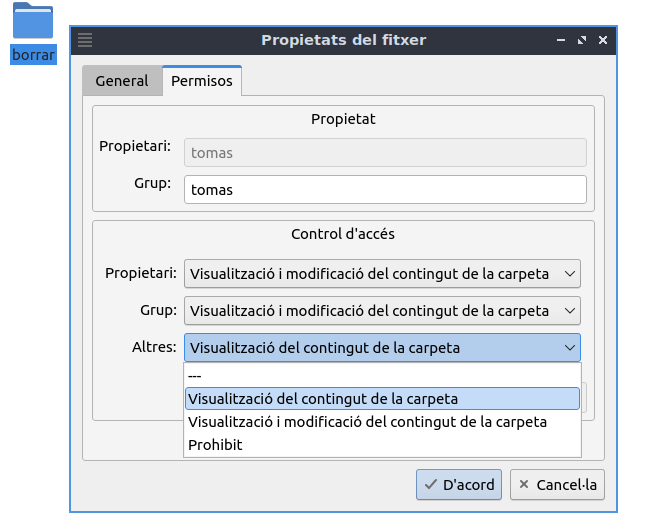
\includegraphics{png/permisosGUIPCManFM-Qt.png}
\caption{\emph{Figura1: Permisos des del GUI (gestor PCManFM-Qt de
Lubuntu)}}
\end{figure}

\subsection{5.2 Limitacions de l'entorn
gràfic}\label{limitacions-de-lentorn-gruxe0fic}

\subsubsection{Permisos
``d'administrador''}\label{permisos-dadministrador}

Crear una carpeta o fitxer si no tens permisos a la carpeta és
impossible. En el CLI, pots fer un ``sudo mkdir\ldots{}'' o ``sudo
touch\ldots{}''

\textbf{Exemple:} Crear una carpeta borrar en \emph{\texttt{/home}}

\begin{figure}
\centering
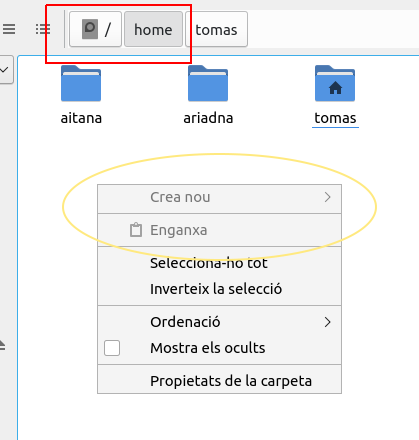
\includegraphics{png/LimitacioGUI.png}
\caption{\emph{Figura2: Falta permisos per crear}}
\end{figure}

Observem que des del CLI, \textbf{amb sudo}

\begin{figure}
\centering
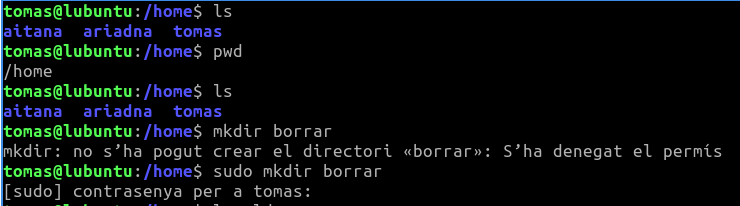
\includegraphics{png/NoLimitacio.png}
\caption{\emph{Figura3: Un usuari sudoer pot crear}}
\end{figure}

Mirem el resultat des dels dos entorns. Fixem-no amb el propietari i
grup assignat.

\begin{figure}
\centering
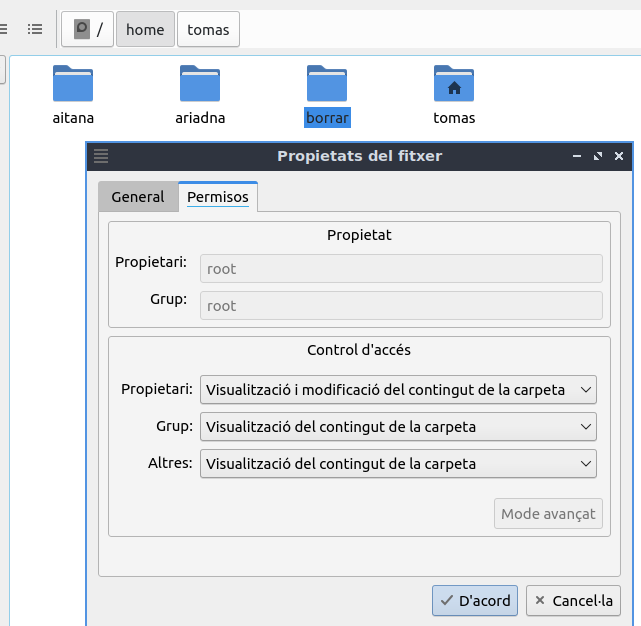
\includegraphics{png/resultatCrearCLIenGUI.png}
\caption{\emph{Figura4: Resultat vist des del GUI (Explorador:
PCManFM-Qt)}}
\end{figure}

\begin{figure}
\centering
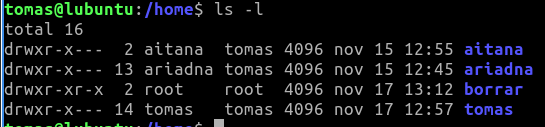
\includegraphics{png/resultatCrearCLIenCLI.png}
\caption{\emph{Figura5: Resultat vist des del teminal}}
\end{figure}

\subsubsection{Diferències entre gestors de
fitxer:}\label{diferuxe8ncies-entre-gestors-de-fitxer}

Depenent del gestor de fitxer que estiguem usant, tindrem més o menys
facilitats. Mireu a la imatge esta comparació entre:

\begin{itemize}
\tightlist
\item
  \textbf{PCManFM-Qt} que ve per defecte en el Lubuntu (part esquerra de
  la imatge)
\item
  \textbf{Thunar} que instal·lem a la Unitat 5 d'este curs (part dreta
  de la imatge)
\end{itemize}

\begin{figure}
\centering
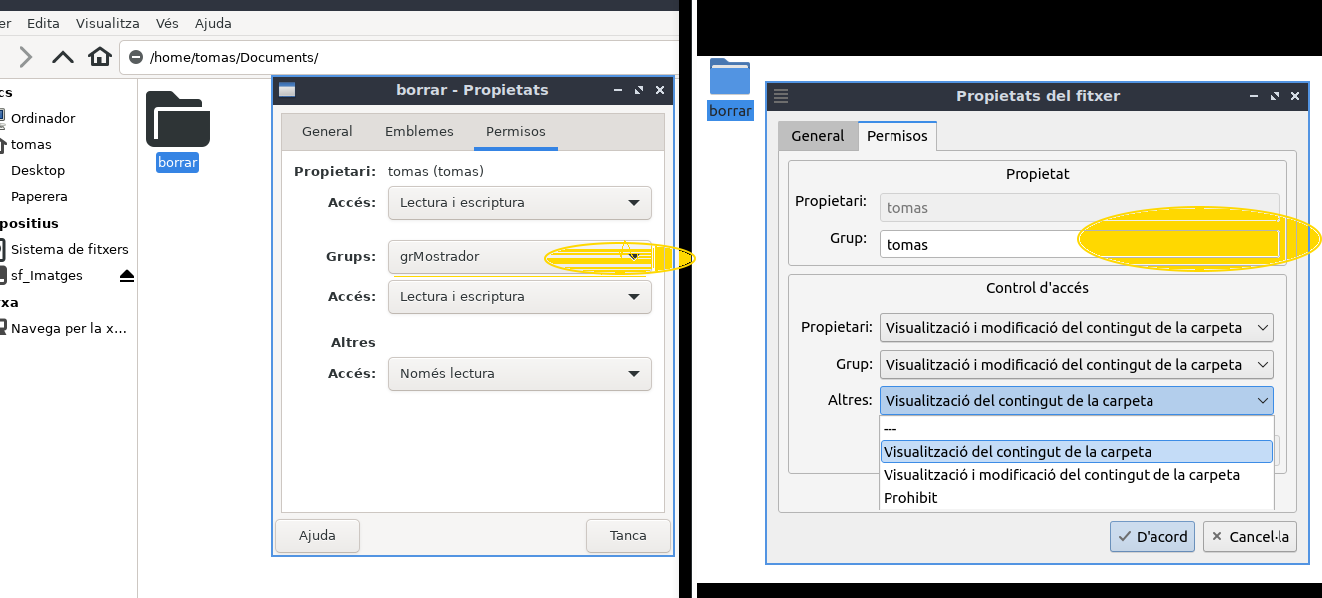
\includegraphics{png/permisosGUIComparativa.png}
\caption{*Figura6:Comparativa entre gestors de fitxers (PCManFM-Qt i
Thunar)}
\end{figure}

També hi ha diverses aplicacions per executar terminals, però una
obertes, les opcions no canvien: un \texttt{ls\ -l}, per exemple sempre
mostra la mateixa informació

\section{6. sudo i propietari}\label{sudo-i-propietari}

Sovint necessitarem crear algun directori o fitxer com a sudoer
(administrador) perquè estem a una carpeta que no tenim permís
d'escriptura. El directori o fitxer que creem tindrà per propietari i
grup a \textbf{root:root}

Depenent del és molt probable que tinguem que fer els canvis de amb
\textbf{chown}.

Dos exemples d'esta casuística que tractarem a les activitats:

\begin{enumerate}
\def\labelenumi{\arabic{enumi}.}
\item
  Un directori del perfil d'un usuari que s'ha eliminat accidentalment (
  /home/joana/Baixades ) i hem de tornar a crear.
\item
  Un directori compartit per als usuaris de la mateixa màquina a
  /home/dadescompartides.
\end{enumerate}

\end{document}
